\documentclass{book}

\usepackage[utf8]{inputenc}
\usepackage[T2A,L7x]{fontenc}
\usepackage[lithuanian,russian]{babel}
\usepackage[svgnames]{xcolor} % Required to specify font color
\usepackage{textcomp}
\usepackage{hyperref}
% \usepackage{fullpage}
\usepackage[shortlabels]{enumitem}
\usepackage{graphicx}
\usepackage{wrapfig}
\usepackage{caption}
\usepackage{nicefrac}
\usepackage{gensymb}

\hypersetup{colorlinks, citecolor=black, filecolor=black, linkcolor=black, urlcolor=black}

\title{25 fotografijos pamokos}
\author{V. P. Mikulinas}
\date{1958}

\renewcommand{\thefigure}{\arabic{figure}}
\addto\captionsrussian{\renewcommand{\partname}{Dalis}}
\addto\captionsrussian{\renewcommand{\chaptername}{Pamoka}}
\addto\captionsrussian{\renewcommand{\figurename}{pieš.}}
\captionsetup[figure]{labelformat=simple, labelsep=space}

\graphicspath{ {/} }

\begin{document}
	\pagenumbering{gobble}% Remove page numbers (and reset to 1)
	\clearpage
	\thispagestyle{empty}

	\maketitle

	\pagebreak
	\cleardoublepage
	\pagenumbering{arabic}% Arabic page numbers (and reset to 1)
	\chapter*{}
	\section*{Autoriaus žodis}
		Fotografija labai paplito moksle, technikoje, visuomeniniame gyvenime, buityje. Fototgrafija --- tarybinės spaudos pagalbininkas; į laikraščius ir žurnalus dedamos nuotraukos supažindina skaitytojus su Tėvynės gyvenimu, rodo mūsų liaudies darbą, kultūrą, poilsį, nušviečia užsienio gyvenimą. Fotografijų mėgėjų skaičius mūsų šalyje pasiekė kelis milijonus.

		Mūsų pramonė kasmet pagamina milijoną fotoaparatų. Trys tūkstančiai aparatų per dieną. Tai reiškia, kad per metus nauji šimtai tūkstančių tarybinių žmonių papildys fotografų mėgėjų eiles.

		Daugeliui pradedančių domėtis fotografija vėliau ji praverčia kasdieniniame darbe --- mokslinėje ekspedicijoje, gamyklos arba instituto laboratorijoje, įmonės arba kolūkio klube ir t. t.. Kai kurie iš jų, gal būt, virs kvalifikuotais fotografais specialistais. Kai kuriems fotografavimas taps patraukliu kultūringu poilsiuarba saviveikliniu menu, kuris artimas dailininkų kūrybai.

		Fotografijos mėgėjai neperšoks per pradinas jos technikos pakopas. Padėti jiems, kiek tai įmanoma, ir ne tik pačioje pradžioje, --- šios knygos uždavinys.

		``25 fotografijos pamokos''  --- ne vadovėlis, o praktiškas vadovas savarankiškai užsiiminėjantiems nespalvotąja fotografija.

		Pirmojoje knygos dalyje išdėstyta tai, kas labiausiai reikalinga pirmai pažinčiai su fotografija --- nuo to momento, kai pradedantis fotografas pirmąkart ima į rankas aparatą, iki gatavo atspaudo padarymo.

		Antrojoje dalyje detalizuojamos pagrindinės fotografinio proceso stadijos. Ši dalis skirta skaitytojams, jau pažįstantiems fotografijos abėcėlę, mokantiems fotografuoti, ryškinti filmą, spausdinti nuotraukas ir norintiems smulkiau studijuoti fotografavimo techniką.

		Trečiojoje dalyje papasakota, kuriuo būdu galima geriausiai nufotografuoti įvairius objektus. Čia išdėstytas kolektyvinis mūsų šalies ir užsienio fotografų patyrimas. Ši dalis skiriama techniškai pasiruošusiems fotografams mėgėjams.

		Kiekvieną ``pamoką'' nebūtina išmokti vienu prisėdimu: ją galima nagrinėti ir savaitę --- kaip kam išeina.

		Suprantama, kad, norint tapti geru fotografu, negana perskaityti knygą. Ji gali duoti pagrindą savarankiškam darbui, išmokyti taisyklingų veiksmų, apsaugoti nuo klaidų, sužadinti norą tobulintis. Visa kita priklauso nuo fotografo mėgėjo atkaklumo ir daugiausia nuo praktikos.

		\textit{Vertėjo pastaba.} Verčiant knygą į lietuvių kalbą, autorius kai kurias teksto vietas pataisė.
	\part{PAGRINDINĖS FOTOGRAFIJOS ŽINIOS}
	\setcounter{section}{0}
	\chapter{Pažintis su fotografija}
	% \section{}
		\textbf{Fotografinio proceso elementai. --- Fotoaparato konstrukcija. --- Medžiagos fotografijai.}
		\section*{Fotografinio proceso elementai}
			Fotografija taip pavadinta, sujungus graikiškus žodžius \textit{photos} (šviesa) ir \textit{grapho} (rašau), ir, išvertus į lietuvių kalbą, reiškia rašymą šviesa, atvaizdų darymą šviesa.

			Šviesos spinduliai, atšokę nuo kokio nors apšviesto daikto ir praėję pro objektyvą, sudaro fotografinės plokštelės (stiklo) arba filmo šviesai jautriame sluoksnyje nematomą \textit{slaptąjį atvaizdą}, kuris po cheminio apdirbimo pavirsta matomu atvaizdu (sudarytu iš atvirkščių tonų) --- \textit{negatyvu}; iš negatyvo daromas ant šviesai jautraus fotografinio popieriaus atspaudas --- \textit{pozityvas}.

			Tokiu būdu, fotografinei nuotraukai padaryti būtini paeiliui trys etapai:
			\begin{enumerate}[1)]
				\item \textit{fotografavimo procesas}, arba fotografavimas (fotografuojamojo daikto atvaizdo ant fotografinės plošktelės arba filmo padarymas fotoaparatu);
				\item \textit{negatyvinis procesas}, arba ryškinimas (cheminis fotografinės plokštelės arba filmo apdirbimas, siekiant paversti slaptąjį atvaizdą matomu --- negatyvu);
				\item \textit{pozityvinis procesas}, arba spausdinimas (galutinio atspaudo ant fotografinio popieriaus padarymas iš negatyvo).
			\end{enumerate}

			\textbf{Fotografavimas.} Norint fotografuoti, reikia turėti prietaisą, kuriuo būtų galima padaryti šviesinį fotografuojamojo daikto atvaizdą ant šviesai jautraus sluoksnio ir kuris kartu apsaugotų šį sluoksnį nuo pašalinės šviesos. Toks prietaisas yra \textit{fotografijos aparatas}. Pagrindinės jo dalys --- šviesos nepraleidžianti \textit{kamera} ir \textit{objektyvas}. Be šių dalių, fotoaparate yra užraktas, reikiamą laiko tarpą atveriąs šviesai kelią į jautrųjį sluoksnį, ir įtaisas keisti atstumui tarp objektyvo ir kameros užpakalinės sienelės. Šis įtaisas leidžia padaryti ryškų atvaizdą daiktų, esančių vienokiu ar kitokiu atstumu nuo aparato; jame yra matinis stiklas arba kitoks prietaisas ryškumui nustatyti.

			Kad būtų vaizdžiau, visą fotografavimo procesą nagrinėsime, taikydami jį plokšteliniams aparatams (``Fotokor'', ``Moskva 3''). Mėgėjai, turintieji filminius fotoaparatus, teperskaito atidžiai (čia ir toliau), kaip veikia plokštelinis aparatas, kaip apdirbama plokštelė, --- tai padės išsiaiškinti procesus, vykstančius fotografimo ir ryškinimo metu. Darbo filminiais aparatais ypatybes vėliau nagrinėsime smulkiai.

			Prieš fotografavimą aparatas išraukiamas, pastatomas ant stovo --- štatyvo (darant momentinę nuotrauką, aparatą galima laikyti rankose), ir objektyvas nukreipiamas į daiktą, kurį numatoma fotografuoti. Paskui atidaromas objektyvas, kuris projektuoja į matinį stiklą sumažintą ir apverstą šviesinį fotografuojamojo daikto vaizdą. Kad šis atvaizdas būtų aiškiau matomas ir kad nekliudytų krintati iš šonų ir iš užpakalio šviesa, kameros užpakalyje yra stogelis. Aparatas pasukamas taip, kad numatytų fotografuoti daiktų atvaizdas tilptų matiniame stikle. Jeigu daiktų atvaizdai dideli ir netelpa, fotografas su aparatu atsitraukia; jeigu jie per maži ir jei norima padaryti didesnį atvaizdą, aparatas priartinamas prie fotografuojamojo daikto.

			Atvaizdas matiniame stikle, tikriausia, bus neryškus, pasklidas. Tada stumiama priekinė aparato dalis į priekį arba atgal (arba sukamas priekinis objektyvo lęšis) tol, kol atvaizdas tampa visiškai ryškus. Tai vadinama \textit{ryškumo nustatymu}.

			Nustačius ryškumą objektyvas uždaromas, išimamas matinis stiklas, ir į jo vietą įstatoma \textit{kasetė} --- tam tikra plokščia šviesos nepraleidžianti dėžutė su ištraukiamu dangteliu. Į kasetę būda įdėta šviesai jautri \textit{plošktelė}. Dabar, atidarius kasetės dangtelį ir objektyvą, į plokštelę projektuosis tas pats atvaizdas, kuris buvo matomas matiniame stikle.

			Fotografuojant ištraukiamas kasetės dangtelis, o paskui paleidžiamas užraktas ir \textit{eksponuojama}, atseit, leidžiama fotografuojamojo daikto šviesiniam atvaizdui tam tikrą apibrėžtą laiką veikti ploštelę, kad jos jautriame sluoksnyje įvyktų pakitimai, po kurių vėliau bus galima gauti pastovų atvaizdą. Paskui kasetės dangtelis įstumiamas, ir kasetė išimama. Tuo fotografavimo procesas baigiamas.

			Tas laiko tarpas, kurį projektuojamas į plokštelę atvaizdas, vadinamas \textit{išlaikymu}. Šis laikas būna labai įvairus --- nuo tūkstantųjų sekundės dalių iki kelių minučių --- ir nustatomas iš pradžių pagal tam tikras lenteles, o paskui, fotografui įpratus, --- iš akies.

			Nufotografavus kasetė kartu su plokštele nunešama į laboratoriją --- tamsų kambarį, apšviestą tam tikra neaktiniška (neveikiančia plokštelės) šviesa. Jeigu kasetė su plokštele būtų nors akimirką atidaryta paprastoje baltoje šviesoje, šviesai jautrus sluoksnis tuojau pat sugestų (nors akis šio pakitimo ir nepastebės). Dėl to reikia rūpestingai saugoti neišryškintas plošteles nuo dirbtinės ar dienos šviesos.\\

			\textbf{Plokštelės ryškinimas.} Atminkite, kad tamsiai raudonoje laboratorijos šviesoje galima apdirbti plokšteles, kurios vazdinamos ``Izoorto'' (ir filmus ``Ortochrom''). Šių plokštelių apdirbimą aprašysime ir toliau.

			Taigi, laboratorijoje, nekenksmingiausioje raudonoje šviesoje, atidaroma kasetė ir išimama plokštelė. Ant jos paviršiaus nematyti jokio atvaizdo: jis kol kas dar nematomas, slaptas, nors fotografuojant, šviesai paveikus, plokštelės fotografiniame sluoksnyje įvyko šiokių tokių pakitimų.

			Kad slaptasis atvaizdas pasidarytų matomas, plokštelė dedama į lėkštą vonelę, į kurią yra įpilta tam tikro tirpalo --- \textit{ryškalo}. Plokštelė vietomis palaipsniuj tamsėja, ant jos pasirodo įvairaus tamsumo juosvai pilkos spalvos vaizdas. Plokštelės šviesai jautrus sluoksnis pakito tose vietose, kurias fotografuojant veikė šviesa. Kuo stipriau veikė šviesa vienas ar kitas plokštelės vietas, tuo labiau jos pakinta ir, vadinasi, tuo labiau patamsėja ryškale. O nuo tamsiųjų fotografuojamojo daikto dalių atšoka į plokštelę maža šviesos, dėl to šios plokštelės vietos  ryškale beveik nepasikeičia, lieka pieniškai gelsvos.

			Slaptojo atvaizdo vertimas matomu vadinamas \textit{ryškinimu}. Ryškinimą reikia baigti, kai visos atvaizdo detalės išryškėja (tam reikia paprastai nuo 4 iki 7 minučių). Jeigu bus ryškinama per ilgai, plokštelė apsitrauks pilkai, apsidengs vualiu.

			Išryškinta plokštelėskaidriai neprasišviečia, yra gelsvo arba rausvo atspalvio ir lieka jautri šviesai. Kad negatyvas pasidarytų visiškai nejautrus šviesai ir skaidrus, kad iš jo vėliau būtų galima spausdinti ant fotografinio popieriaus, jis, paskalautas vandenyje, paneriamas į kitą tirpalą --- \textit{fiksažą}. Iš fiksažo negatyvas išimamas, kai šviesiosios vietos tampa visiškai skaidrios (fiksavimas trunka 10 -- 15 minučių). Po to negatyvas rūpestingai plaunamas vandenyje ir džiovinamas.

			Kaip jau kalbėta, plokštelę ryškinti reikia nekenksmingoje raudonoje šviesoje. Praėjus kelioms minutėms nuo fiksavimo pradžios, laboratorijoje jau galima įžiebti baltą šviesą --- ji plokštelei nebekenkia.

			Ryškinimas ir fiksavimas kartu vadinami \textit{negatyviniu procesu}. Po šio proceso gauname \textit{negatyvą}, kuriame yra fotografuoto daikto atvaizdas, bet su atvirkščiu šviesių ir tamsių vietų išdėstymu: tamsiosios nufotografuoto daikto vietos čia yra šviesios (net ir skaidrios), o šviesiosios daikto vietos čia tamsios (net ir nepermatomos). Negatyvinis atvaizdas yra tarpinis.\\

			\textbf{Atspaudo ant fotografinio popieriaus darymas.} Galutinis fotografavimo tikslas yra padaryti nufotografuoto daikto teisingų tonų atvaizdą. Tuo tikslu išdžiovintas negatyvas uždedamas ant šviesai jautraus fotografinio popieriaus ir apšviečiamas. Šviesa, praėjusi pro negatyvą, veikia fotografinį popieriaus sluoksnį . Kuo tamsesnės atskiros negatyvo vietos, tuo mažiau šviesos jos praleidžia, ir dėl to po tamsiomis negatyvo vietomis šviesa veikia silpnai, po šviesiomis --- stipriau.

			Fotografijos praktikoje naudojami beveik išimtiniai ryškinamieji fotografiniai popieriai, kuriuose atvaizdas išeina nematomas (slaptas), kaip ir plokštelėje fotografavimo metu. Atvaizdą reikia išryškinti, kad jis pasidarytų matomas --- sudarytas iš tonų, atvirkščių negatyvui, ir atitinkąs fotografuotąjį daiktą. Paskui atspaudas fiksuojamas, plaunamas ir džiovinamas. Šie fotografiniai popieriai apdirbami taip pat kaip ir plokštelės negatyviniame procese, tamsiame kambaryje, bet šviesesnėje --- oranžinėje arba šviesiai raudonoje šviesoje.

			Atspaudas ant fotografinio popieriaus vadinamas \textit{pozityvu}, o jo gavimo iš negatyvo operacijos --- \textit{pozityviniu procesu}.

			Atspaudą ant fotografinio popieriaus galima padaryti ne tik aprašytuoju \textit{kontaktiniu} būdu, kurio atspaudas padaromas tokio pat dydžio kaip ir negatyvas, bet ir \textit{projekciniu} spausdinimo būdu, vadinamuoju \textit{fotografiniu didinimu}. Spausdinant šiuo būdu, padidintas negatyvinis atvaizdas projektuojamas tamsiame kambaryje projekciniu žibintu į šviesai jautrų popierių (panašiai, kaip projektuojamas filmas kine į ekraną).

			Trumpai susipažinę, kaip vyksta pagrindiniai fotografinio proceso etapai, pradėsime nagrinėti smulkiau, praktiškai, kiekvieną iš jų atskirai.

			Ši knyga skirta paprastos juodos-baltos fotografijos procesams. Spalvotosios fotografijos ji neliečia. Daugiasluoksnių spalvotųjų fotografibių medžiagų apdirbimas, ypač spalvotųjų pozityvų darymas ant popieriaus, žymiai sudėtingesnis už atitinkamus juodos-baltos fotografijos procesus. Fotografas mėgėjas gali pereiti prie spalvotosios fotografijos tik po to, kai išmoksta paprasto fotografavimo technikos. O pagal principinę schemą abi fotografijos rūšys yra vienodos.
		\section*{Fotoaparato konstrukcija}
			Susipažinsime iš pradžių, kaip sudarytas fotografijos aparatas, kuriuo padaromas šviesinis (optinis) atvaizdas.
			\subsection*{Pagrindinės fotografijos aparato dalys}
				Žiūrint paskirties ir konstrukcijos, fotografijos aparatai turi vienokius ar kitokius prietaisus, skirtus fotografavimo operacijoms suprastinti, palengvinti ir patikslinti, bet sudaryti jie visi pagal vieną principą. Fotografavimo proceso esmė visada lieka ta pati: objektyvas projektuoja kameroje fotografuojamojo daikto optinį atvaizdą, kuris atsispaudžia ant šviesai jautrios plokštelės arba filmo.

				Šių laikų bendros paskirties fotografijos aparatas sudarytas iš šių pagrindinių dalių: 1) kameros (šviesos nepraleidžiančios dėžtuės); 2) objektyvo (prietaiso optiniam atvaizdui sudaryti); 3) užrakto (mechanizmo, kuriuo šviesinis atvaizdas reikiamą laiko tarpą praleidžiamas į plokštelę arba filmą); 4) mechanizmo ryškumui nustatyti; 5) vaizdo ieškiklio (prietaiso fotoaparatui nutaikyti į fotografuojamąjį objektą).

				Būtinas fotoaparato priedas yra kasetė (arba kitoks prietaisas jautriajai fotografinei medžiagai įdėti).
				\subsubsection*{Kamera}
					Kamera, paprastai kalbant, yra šviesos nepraleidžianti dėžutė, kurios vienoje sienelėje įtvirtintas objektyvas, o priešingoje sienelėje įtaisoma šviesai jautri medžiaga (1 pieš.).
					\begin{figure}[h]
						\centering
						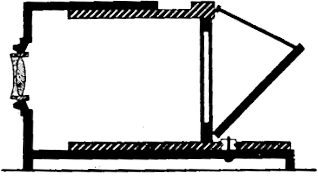
\includegraphics[width=0.8\textwidth]{1-pav}
						\caption{Pirmojo pardavinėjimui skirto fotoaparato pjūvis (Dager, 1839 m. Nuo to laiko kameros schema nepasikeitė)}
						\label{fig:1}
					\end{figure}
					Kamera turi apsaugoti fotografinę plokštelę arba filmą nuo bet kokios pašalinės šviesos. Fotoaparatų kameros arba korpusai būna: a) standūs, dėžutės tipo (``Liubitel''); b) standūs kompaktiški su ištraukiamu objektyvu (FED, ``Zorkij'', ``Kijev''); c) su sustumiamomis dumplėmis, siaurėjančiomis (``Fotokor'', ``Moskva'') arba vienodo skerspjūvio (štatyvinės kameros), panašiomis į armonikos dumples.

					Konstruktoriai stengiasi padaryti tokią kamerą, kuri suglausta užimtų kuo mažiau vietos.
				\subsubsection*{Objektyvas}
					Svarbiausia fotoaparato dalis --- objektyvas. Tai yra optinis prietaisas, projektuojąs į plokštelę arba filmą fotografuojamojo daikto šviesinį atvaizdą.
					\begin{wrapfigure}{r}{0.33\textwidth}
						\centering
						
\includegraphics[width=0.33\textwidth]{2-pav}
						\caption{Pusiau suklijuoto keturių lęšių anastigmato ``Industar'' konstrukcinė schema}
						\label{fig:2}
					\end{wrapfigure}
					Paprastas surenkamas lęšis (didinamasis stiklas) duoda pasklidą, neryškų atvaizdą. Dėl to objektyvai, kurie dabar naudojami fotografijoje, paprastai yra sudaryti iš kelių (nuo trijų iki aštuonių) lęšių, kurių iškilumas arba įdubimas (kreivumo spinduliai) ir stiklo sudėtis tiksliai apskaičiuoti ir išlaikyti gaminant. Gretimi lęšiai atskiriami oro tarpu arba suklijuojami. Tokie tobuli objektyvai vadinami \textit{anastigmatais}; jie duoda aiškų ir ryškų atvaizdą. Visuose mūsų šalyje gaminamuose fotoaparatuose įstatyti anastigmatai (2 pieš.).

					Objektyvas montuojamas įtvare, atitinkančiame kamerą, kuriai jis skirtas. Aparatų su centriniu užraktu objektyvai įmontuoti įtvare, kuris sujungtas su užraktu; mažojo formato aparatų objektyvai --- dvigubame įtvare su sriegiais, kurių dėka objektyvą galima pastumti (sukant) išilgai optinės ašies ir tuo nustatyti atvaizdo ryškumą; štatyvinių kamerų objektyvų įtvarai vadinami normaliais įtvarais.

					Ant objektyvo įtvaro išgraviruota: vienos ar kitos rūšies objektyvo pavadinimas, jo židinio nuotolis ir santykinė anga (šviesos stiprumas), o kai kada ir gaminusio fabriko markė bei eilės numeris. Ten pat arba ant centrinio užrakto įtvaro padaryta diafragmų skalė, o daugumoje šiuolaikinių objektyvų --- ir atstumų skalė bei ryškumo zonos skalė.

					Židinio nuotolis ir santykinė anga yra pagrindiniai objektyvą apibūdinantieji duomenys.\\
				
					\textbf{Židinio nuotolis.} Židinio nuotoliu (pagrindiniu) vadinamas atstumas tarp objektyvo optinio centro ir plošktelės (arba filmo), kai ryškiai nustatytas labai tolimo daikto atvaizdas. Jeigu objektyvas nustatytas taip, kad labai tolimų daiktų (pavyzdžiui, trobesio ir kt., esančių ne arčiau kaip už 100 \textit{m} nuo aparato) atvaizdas matiniame stikle išeina ryškus (tai vadinama ryškumo nustatymu begalybei), tai atsumas tarp objektyvo diafragmos plokštumos ir matinio stiklo yra lygus to objektyvo židinio nuotoliui\footnote{Tai galioja objektyvams, kurių diafragmos plokštuma eina per optinį centrą. Daugumai objektyvų tas atstumas tik apytikriai bus lygus objektyvo židinio nuotoliui. Teleobjektyvams šios taisyklės taikyti negalima.}. Kiekvieno objektyvo židinio nuotolis --- tai tas mažiausias atstumas nuo jo optinio centro iki plokštelės, kuriuo tegalima gauti ryškų atvaizdą. Fotografuojant arčiau esančius daiktus, atstumą tarp objektyvo ir plokštelės tenka padidinti; norint daiktą nufotografuoti natūralaus didumo (neperžengiant aparato plokštelės dydžio ribų), reikėtų dumples ištempti dvigubu objektyvo židinio nuotolio dydžiu --- reikėtų panaudoti \textit{dvigubo ilgio} dumples. Iš mūsų šalyje masiškai gaminamų fotoaparatų tiktai ``Fotokor'' turi dvigubo ilgio dumples; dėl to kitais aparatais negalima fotografuoti labai arti (arčiau kaip už 1,3 -- 1,5 \textit{m}) esančių daiktų, nepanaudojus papildomų prietaisų.

					Židinio nuotolis išreiškiamas centimetrais (arba milimetrais). Nuo jo dydžio priklauso objektyvo šviesos stiprumas ir ryškiai atvaizduojamos erdvės zona, daiktų atvaizdų mastelis ir, be to, kiekvienai objektyvo konstrukcijai --- didžiausias plokštelės arba filmo formatas, kuriuo galima padaryti iki kraštų ryškų atvaizdą.

					Fotografuojant iš to paties taško, objektyvas su trumpu židinio nuotoliu duoda mažo formato atvaizdą smulkiu masteliu, objektyvas su ilgu židinio nuotoliu duoda didelio formato atvaizdą stambiu masteliu. Atvaizdų mastelis yra tiesiog proporcingas židinių nuotoliams.

					Normaliais židinių nuotoliais laikomi: 9 \texttimes 12 \textit{cm} negatyvui --- 13,5 centimetro; 6 \texttimes 9 \textit{cm} negatyvui --- 11 centimetrų; 6 \texttimes 6 cm negatyvui --- 7,5 centimetro; mažojo formato negatyvui (24 \texttimes 36 mm) --- 5 centimetrai.\\

					\textbf{Santykinė anga (geometrinis šviesos stiprumas).} Objektyvo šviesos stiprumu vadinama jo galia apšviesti vienokiu ar kitokiu stiprumu kameroje esančios fotografinės medžiagos šviesai jautrų sluoksnį. Šviesos stiprumo dydžio reikšmė didelė: kuo didesnis objektyvo šviesos stiprumas, tuo mažesnio išlaikymo (plokštelės arba filmo apšvietimo laiko) reikia fotografuojant.

					Suprantama, kad objektyvas su didele anga praleidžia daugiau šviesos negu objektyvas su maža anga. Tačiau absoliutus objektyvo skersmens dydis dar nieko nenuliame. Iš tikrųjų: jeigu palyginsime objektyvą su langu, pro kurį į tamsią patalpą (kamerą) patenka šviesa, tai nesunkiai įsitikinsime, kad bet kuris daiktas (plokštelė arba fimas) bus apšviestas tuo stipriau, kuo didesnis pats langas ir kuo arčiau yra tas daiktas.

					Vadinasi, objektyvo šviesos stiprumas priklauso nuo dviejų dydžių: nuo angos dydžio ir nuo židinio nuotolio. Objektyvo šviesos stiprumas tuo didesnis, kuo didesnė jo anga ir kuo trumpesnis jo židinio nuotolis.

					Šis ryšys išreiškiamas \textit{santykinės angos} dydžiu, kuris yra santykis tarp pilnos objektyvo veikančiosios angos\footnote{Pilna veikiančiąja anga vadinama didžiausia objektyvo anga (įeinamasis vyzdys), pro kurią praeina šviesos spindulių pluoštas; ji paprastai lygi pirmajam lęšiui arba kiek mažesnė už jį (išimtis --- plačiakampiai objektyvai).} skersmens ir jo pagrindinio židinio nuotolio (žinoma, abu dydžiai imami vienodais ilgio vienetais). Pavyzdžiui, angos skersmuo (2 \textit{cm}) sutinka su židinio nuotoliu (8 \textit{cm}) kaip 2 : 8; po suprastinimo (padalijus santykį iš pirmojo nario dydžio) gaunama 1 : 4 --- tai ir yra santykinės angos skaitinė reikšmė.

					Fotoaparato FED objektyvo pilnos angos skersmuo 14,3 \textit{mm}, židinio nuotolis 50 \textit{mm}, o padaliję iš pirmojo nario dydžio (14,3), gausime 1 : 3,5.

					Santykinė anga žymima santykiu tarp vieneto ir skaičiaus, rodančio, kiek kartų to objektyvo pilnos angos skersmuo mažesnis už jo židinio nuotolį.

					Šiuolaikiniuose aparatuose būna objektyvai su santykinėmis angomis 1 : 1,5; 1 : 2; 1 : 2,8; 1 : 3,5; 1 : 4; 1 : 4,5; 1 : 6,3. Kuo didesnis antrasis santykio narys, tuo mažesnė pati santykinė anga. Tai suprantama: santykinės angos skaitinė reikšmė yra trupmena. O kadangi \nicefrac{1}{4} yra mažiau už \nicefrac{1}{2}, tai ir santykinė anga 1 : 4 yra mažesnė už angą 1 : 2.

					Objektyvo anga --- tai skritulys; kaip žinome iš geometrijos, skritulių plotai sutinka kaip jų skersmenų kvadratai. Vadinasi, vieno objektyvo šviesos stiprumas sutinka su kito šviesos stiprumu kaip atitinkamų santykių angų skersmenų kvadratai. Tačiau yra paprastesnis būdas nustatyti, kiek kartų vieno objektyvo šviesos stiprumas didesnis už antrojo: didesnįjį dviejų santykinių angų vardiklį reikia padalyti iš mažesniojo vardiklio ir gautą dalmenį pakelti kvadratu (padauginti patį iš savęs). Pavyzdys: sulyginamas šviesos stiprumas objektyvų, kurių santykinės angos 1 : 4,5 ir 1 : 1,5.
					\[
						(4,5 : 1,5)^{2} = 3^{2} = 9.
					\]

					Vadinasi, antrojo objektyvo šviesos stiprumas yra 9 kartus didesnis už pirmojo, ir, kai anga visa atidaryta, viendomis fotografavimo sąlygomis antrajam objektyvui reikia 9 kartus mažesnio išlaikymo (suapvalinus, pavyzdžiui, \nicefrac{1}{100} sekundės vietoj \nicefrac{1}{10} sekundės).

					\textbf{Diafragma.} Ant objektyvo (apatinėje centrinio užrakto dalyje arba tiesiog ant įtvaro) yra eilė didėjančių skaičių, pavyzdžiui, tokių: 4,5 --- 5,6 --- 8 --- 11 --- 16 --- 22 --- 32 (``Moskva'') arba 3,5 --- 4,5 --- 6,3 --- 9 --- 12,5 --- 18 (FED), kurių pirmasis visada sutampa su objektyvo santykinės angos vardikliu.

					Atidarę centrinį užraktą ir nustatę esančią prie skaitmenų rodyklę-slankiklį ties mažiausiu skaičiumi, pamatysime, kad objektyvo anga atidaryta visa. Jeigu slankiklį stumsime didesnių skaičių link, objektyvo anga palaipsniui mažės ir ties didžiausiu skaičiumi bus mažiausia. Prietaisas objektyvo angai reguliuoti vadianamas \textit{diafragma}, o skaičių eilė --- tai šio prietaiso skalė.

					Šių laikų objektyvuose naudojama vadinamoji irisinė diafragma; ji sudaryta iš lapelių, esančių tarp objektyvo lęšių (maždaug jo optinio centro plokštumoje) ir sudarančių beveik apskritą angą. Susieidami arba prasiskirdami, lapeliai palaipsniui keičia objektyvo veikiančiosios angos dydį (3 pieš.).

					Skaičiai diafragmų skalėje yra objektyvo faktinių (veikiančiųjų) santykių angų vardikliai įvairioms slankiklio padėtims. Jie apskaičiuojami tuo pačiu principu, kaip ir pilna santykinė anga, bet skaitiklis, visada lygus vienetui, patogumo dėlei nežymimas (4 pieš.).

					Diafragma vadinama ir pati reguliuojamoji anga, žymint jos dydį atitinkamu skaitiniu rodikliu (diafragma 5,6) arba išreiškiant jį žodžiais (didelė diafragma, maža diafragma).
					\begin{figure}[h]
						\centering
						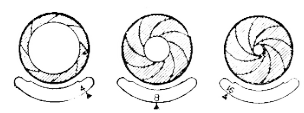
\includegraphics[width=0.8\textwidth]{3-pav}
						\caption{Irisinė diafragma}
						\label{fig:3}
					\end{figure}
					\begin{figure}[h]
						\centering
						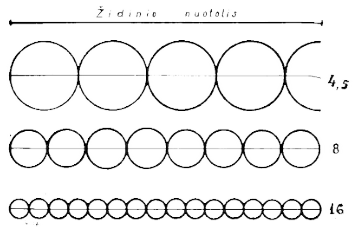
\includegraphics[width=0.8\textwidth]{4-pav}
						\caption{Diafragmos kiekvienos angos dydis žymimas skaičiumi, kuris rodo, kiek kartų angos skersmuo telpa objektyvo židinio nuotolyje}
						\label{fig:4}
					\end{figure}
					Pastaruoju atveju turimas galvoje angos dydis, bet ne skaičius, kuriuo ta anga pažymėta skalėje. Didelė diafragma --- tai didelė anga, bet maži skaičiai (1,5 -- 4,5). Maža diafragma --- tai maža anga, bet dideli skaičiai (11 -- 36). Vidutinė diafragma --- tai 5,6 -- 9\footnote{Diafragmos anga visais atvejais laikoma veikiančioji objektyvo anga. Ji lygi šiek tiek padidintam diafragmos vaizdui, matomam pro priekinį lęšį. 2 V. P. Mikulinas}.

					Kad būtų trumpiau, sutarsime toliau (tik šioje knygoje) objektyvo šviesos stiprumo dydį žymėti vien tik pilnosios santykinės angos vardikliu, panašiai kaip žymima diafragmų skalėje.

					Siaurindamas objektyvo praleidžiamų šviesos spindulių pluoštą, diafragmavimas sumažina plokštelės arba filmo apšvietimo laipsnį, ir dėl to jau reikia pailginti išlaikymą fotografuojant. Kuo mažesnė naudojamoji diafragmos anga, tuo ilgesnis turi būti išlaikymas.

					Reikia atminti, kad, pavyzdžiui, diafragmos 4 anga visai ne 2 kartus mažesnė už diafragmos 2 angą, bet 4 kartus, ir dėl to išlaikymo su šia diafragma reikia ne du, bet keturis kartus ilgesnio.
					\begin{figure}[h]
						\centering
						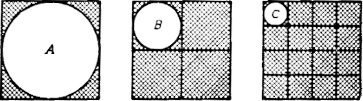
\includegraphics[width=0.8\textwidth]{5-pav}
						\caption{Sumažėjus skritulio skersmeniui 2 kartus, skritulio plotas sumažėja $2^{2}$, atseit, keturis, kartus. Skritulių $A$, $B$ ir $C$ skersmenys sutinka kaip 1 : \nicefrac{1}{2} : \nicefrac{1}{4}, o jų plotai kaip 1 : \nicefrac{1}{4} : \nicefrac{1}{16}}
						\label{fig:5}
					\end{figure}
					Tai paaiškinama tuo, kad diafragmos angos numeruojamos pagal jų skersmenis, o apskritų angų plotai sutinka kaip skersmenų kvadratai. Dėl to, sumažėjus 2 kartus angos skersmeniui, jos plotas sumažėja $2^{2} = 4$ kartus.

					Šį santykį vaizdžiai paaiškina 5 piešinys. Nesunku įsitikinti, kad vidurinio skritulio $B$ skersmuo lygiai du kartus mažesnis už kairiojo skritulio $A$ skersmenį; tuo tarpu jo plotas keturis kartus mažesnis, ir, vadinasi, anga $B$ praleis šviesos 4 kartus mažiau negu anga $A$. Dešiniojo skritulio $C$ skersmuo yra 4 kartus mažesnis už kairiojo skritulio $A$ skersmenį, o jo plotas 16 kartų mažesnis. Tas pats ir su diafragmos angomis.

					Kintamų diafragmų skalė sudaryta taip, kad kiekvienai gretimai diafragmai išlaikymo reikia dukart ilgesnio (jeigu anga sumažinama) arba dukart trumpesnio (jeigu anga padidinama)\footnote{Išimtis daroma tiktai pilnajai angai, kai jos dydis neįeina į standartinę diafragmų eilę.}. Tokiu būdu, sumažinus angą per dvi skalės padalas, išlaikymas paketurgubėja ir t. t.

					Žemiau, 1 lentelėje, parodoma (šiek tiek apvalinti) dafragmų angų ir reikalingų išlaikymų priklausomybė.
					\begin{table}[h]
						\caption{\textbf{Priklausomybė tarp diafragmos ir išlaikymo}}
						\begin{tabular}{c|c|c|c|c|c|c|c|c|c|c|}
							\hline
							Diafragma & $\frac{1,4}{1,5}$ & 2 & 2,5 & 2,8 & 3,5 & 4 & 4,5 & 5,6 & 6,3 & 6 \\ \hline
							Santykinis išlaikymo dydis & 1 & 2 & 3 & 4 & 6 & 8 & 10 & 16 & 20 & 32 \\
							\hline
						\end{tabular}
						\begin{tabular}{c|c|c|c|c|c|c|c|c|c|}
							\hline
							Diafragma & 9 & 11 & 12,5 & 16 & 18 & 22 & 25 & 32 & 36 \\ \hline
							Santykinis išlaikymo dydis & 40 & 64 & 80 & 128 & 160 & 256 & 320 & 512 & 640 \\
							\hline
						\end{tabular}
					\end{table}

					Iš lentelės matyti, kad diafragmai 32 reikia 50 kartų ilgesnio išlaikymo negu diafragmai 4,5 ir maždaug 500 kartų ilgesnio išlaikymo negu pilnai objektyvo angai 1,5. Jeigu objektyvas, kurio šviesos stiprumas 2, diafragmuojamas iki 5,6, tai išlaikymą reikia pailginti 8 kartus (16 : 2).

					Diafragmų (vadinasi, ir išlaikymų) reikšmės yra vienodos bet kuriems objektyvams, nepriklausomai nuo jų konstrukcijos, židinio nuotolio ir pilno šviesos stiprumo. Jeigu dviejuose objektyvuose, iš kurių vieno švieos stiprumas 1,5, kito --- 4,5, nustatysime diafragmą 8, tai fotografuojant abiem atvejais išlaikymo reikia vienodo\footnote{Geometrinio šviesos stiprumo požiūriu.}.

					Kam gi reikalinga išlaikymą ilginanti diafragma? Žinoma, ne tiktai atvaizdui ant plokštelės ar filmo patamsinti, nors objektyvo praleidžiamos šviesos sumažinimas būna naudingas, kai objektas nušviestas skaisčios saulės, negatyvinė medžiaga labai jautri, objektyvo šviesos stiprumas didelis, trumpiausiasis užrakto automatiškai atliekamas išlaikymas per ilgas, ir be diafragmavimo būtų neišviangiamas negatyvo peršvietimas (perlaikymas).

					Pagrindinė diafragmavimo paskirtis yra gauti ryškų atvaizdą, praplečiant vidanamąją ryškiai vaizduojamos erdvės zoną tais atvejais, kai norima viename negatyve nufotografuoti iš karto objektus, esančius įvairiais atstumais nuo aparato (vieni arti, kiti toliau arba labai toli).

					\textit{Apie praskaidrintuosius objektyvus.} Daugumas mūsų šalyje gaminamų fotoobjektyvų yra praskaidrinti, kitaip sakant, juose sumažintas kiekis šviesos, kuri paprastai atšoka ir išsisklaido nuo lęšių paviršių ir dėl to arba nepasiekia plokštelės ar filmo, arba sukuria vualį. Paskaidrinimas padidina atvaizdo kontrastą, maždaug 30\% sumažina išlaikymą. Be to, paskaidrintas objektyvas sumažina aureolių susidarymą, duoda švaresnį atvaizdą, kai fotografuojama prieš šviesą ir fotografuojant objektus su smarkiai atspindinčiais paviršiais (sniegas saulėje, vanduo, stiklas ir pan.). Objektyvai paskaidrėja, aptraukus lęšių poliruotus paviršius, susisiekiančius su oru, mikroskopiškai plonu skaidriu sluoksniu, kuris suteikia jiems violetiškai melsvą atspalvį. Kad būtų galima įsivaizduoti skaidrinančio sluoksnio storį, pažymėsime, kad jis lygus \nicefrac{1}{1000} paprastos filminės juostelės storio.

					Tai ir visos žinios apie objektyvą, reikalingos pradedančiajam fotografui mėgėjui iš pradžių, juo labiau, kad jau gamykloje į kiekvieną fotoaparatą įdedamas trumpiausias objektyvas, ir rinktis jo nebereikia.
				\subsubsection*{Užraktas}
					Fotografinis užraktas --- mechanizmas, kuris atidaro praėjusiems pro objektyvą šviesos spinduliams kelią į plokštelę arba filmą ir po tiksliai nustatomo laiko tarpo uždaro jį. Užraktu daromas trumpas išlaikymas, kuris dabartinėje fotografijoje (pavyzdžiui, fotografuojant greitai judančius objektus) trunka šimtąsias ir tūkstantąsias sekundės dalis.

					Mėgėjiškuose aparatuose pasitaiko dvejopų užraktų: 1) centrinis užraktas, atidarąs ir uždarąs veikiančiąją objektyvo angą (jis įtaisytas mūsų aparatuose, skirtuose plošktelėms ir plačiam filmui); 2) užuolaidinis užraktas, atidengiąs ir uždengiąs negatyvinės medžiagos plokštumą (jis įtaisytas mūsų mažojo formato filminiuose aparatuose).

					\textit{Centrinis užraktas} taip pavadintas pagal savo veikimo principą. Jo dalis, užstojanti šviesą, yra sudaryta iš kelių metalinių ploštelių-sąvarėlių, esančių tarp lęšių. Ši dalis pradeda objektyvo atidarymą ir baigia jo uždarymą veikiančiosios angos centre. Visa plokštelė apšviečiama vienu metu. Šis užraktas, tikslus laikrodinis mechanizmas, įtaisomas žiedu aplink objektyvą ir sujungiamas su objektyvo įtvaru. Mūsų šalyje gaminami centriniai užraktai automatiškai išlaiko atidarytą objektyvą nuo 1 iki \nicefrac{1}{250} sekundės.

					\textit{Užuolaidinis užraktas} taip pavadintas dėl savo šviesą užstojančios detalės --- šviesos nepraleidžiančios \textit{užuolaidėlės}, kuri sudaryta iš dviejų dalių, atskirtų skersiniu plyšiu. Užuolaidėlė padaryta iš gumuotos šilkinės medžiagos arba sudaryta iš siaurų skersinių metalinių juostelių. Užraktas įmontuotas į fotoaparato korpusą. Veikimo metu užuolaidėlė, persivyniodama nuo vieno velenėlio ant kito, pralekia palei patį filmą, kuris pro užuolaidėlės plyšį apšviečiamas palaipsniui nuo vieno krašto iki kito. Tokie užraktai automatiškai atmatuoja išlaikymą nuo 1 iki \nicefrac{1}{1250} sekundės (išlaikymo dydis reguliuojamas, keičiant plyšio plotį ir užuolaidėlės pralėkimo greitį).

					Tokiu būdu, žemutinė mūsų gaminamų užuolaidinių užraktų išlaikymo riba yra 5 kartus mažesnė negu centrinių užraktų. Abiejų tipų užraktais galima laikyti objektyvą atidarytą kiek patinka, laikant nuspaustą užrakto svirtelę (mygtuką).

					Užraktas --- sudėtingiausia fotoaparato dalis; naudotis juo reikia išmokti tobulai, stebint jo veikimą ant matinio stiklo pro atidarytą užpakalinę kameros sienelę arba iš priekio pro objektyvą.

					Kaip pavyzdį išnagrinėsime, kaip veikia centrinis užraktas ``Moment'' (6 pieš.), kuris įtaisomas fotoaparatuose ``Moskva''. Patogiausia jo darbą stebėti ant aparato ``Moskva 3'' matinio stiklo.

					Atidarę aparatą, atlenkiame stogelį, esantį už matinio stiklo. Jeigu dabar nukreipsime objektyvą į apšviestą langą, tai ant matinio stiklo dar nieko nepamatysime, nes užraktas uždarytas. Norint atidaryti užraktą, reikia iš pradžių pasukti žiedą --- išlaikymo reguliatorių taip, kad raidė \textit{Д} atsidurtų ties rodykle viršutinėje užrakto dalyje; nuspaudus užrakto svirtelę (arba mygtukinę žarnelę), užraktas atsidaro.

					Jeigu dabar, atleidę svirtelę, nukreipsime objektyvą į langą, tai kameros matinis stiklas nušvis.
					\begin{figure}[h]
						\centering
						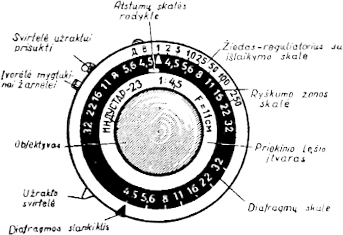
\includegraphics[width=0.8\textwidth]{6-pav}
						\caption{Centrinis užraktas ``Moment''}
						\label{fig:6}
					\end{figure}
					Jeigu vėl paspausime užrakto svirtelę, užraktas užsidarys, ir matinis stiklas vėl pasidarys tamsus. Tokiu būdu, kai reguliatorius nustatytas ties raide \textit{Д}, pirmuoju svirtelės paspaudimu užraktas atidaromas, antruoju paspaudimu --- uždaromas. Taip užraktas nustatomas, fotografuojant ilgu išlaikymu (ilgesniu kaip 5 sekundžių).

					Jeigu ties rodykle nustatysime išlaikymo reguliatoriaus raidę \textit{B}, tai atvaizdas ant matinio stiklo bus matomas tik tol, kol užrakto svirtelė laikoma nuspausta. Kai tik jūs atleisite svirtelę, užraktas užsidarys. Taip užraktas nustatomas, fotografuojant trumpesniu išlaikymu (nuo 1 iki 5 sekundžių).

					Pagaliau, jeigu ties rodykle nustatysime kurį nors iš skaitmenų, esančių išlaikymo reguliatoriaus skalėje (nuo \textit{1} iki \textit{250}) ir žyminčių sekundės dalis, o paskui pasuksime užraktą, pasukę jo prisukamąją svirtelę į dešinę iki galo, tai, paspaudus užrakto svirtelę, atvaizdas ant matinio stiklo pasirodys atitinkamą trumpą laiko tarpą ir tuojau pat išnyks. Taip užraktas ``Moment'' nustatomas, fotografuojant 1 -- \nicefrac{1}{250} sekundės išlaikymu (2 lent.).
					\begin{table}[h]
						\caption{\textbf{Priklausomybė tarp diafragmos ir išlaikymo}}
						\begin{tabular}{c|c}
							\hline
							Reguliatoriaus išlaikymas & Naudojimas ir veikimas \\ \hline
							Д & \textbf{Nustatant ryškumą pagal matinį stiklą. Fotografuojant ilgu išlaikymu (ilgesniu kaip 5 sekundės)} \par Pirmą kartą paspaudus užrakto svirtelę (arba mygtukinę žarnelę), užraktas atsidaro ir lieka atviras tol, kol užrakto svirtelė paspaudžiama pakartotinai \\ \hline
							B & \textbf{Fotografuojant trumpu išlaikymu (nuo 1 iki 5 sekundžių)} \par Užraktas atviras tol, kol laikoma nuspausta užrakto svirtelė. Atleidus svirtelę, užraktas užsidaro. \\ \hline
							1, 2, 5, 10, 25, 50, 100, 250 & \textbf{Fotografuojant užrakto automatiškai reguliuojamu išlaikymu} \par \textit{Nustačius išlaikymo reguliatorių, užraktą reikia prisukti} \par Paspaudus užrakto svirtelę, užraktas atsidaro ir po atitinkamos sekundės dalies (1 sekundė, \nicefrac{1}{2}, \nicefrac{1}{5}, \nicefrac{1}{10}, \nicefrac{1}{25}, \nicefrac{1}{50}, \nicefrac{1}{100} arba \nicefrac{1}{250} sekundės) automatiškai užsidaro \\
						\end{tabular}
					\end{table}

					Fotografuojant nuo štatyvo (tai būtina, kai išlaikymas ilgesnis kaip \nicefrac{1}{20} sekundės), užraktą reikia paleisti, paspaudžiant mygtukinę žarnelę, įsukamą į užrakto mygtuko skylutę.

					Filminių fotoaparatų centriniuose užraktuose nėra padalos \textit{Д} (kad pro atvirą objektyvą atsitiktinai nepatektų šviesos į pervniotą filminę juostelę).

					Mažojo formato aparatų užuolaidiniuose užraktuose padalos \textit{Д} taip pat nėra (išimtis --- ``Zorkij 3''); senuose aparato FED modeliuose padalą \textit{B} atstoja padala \textit{Z}.

					Kad nesugestų mechanizmai, išlaikymą keisti reikia tiktai tada, kai centrinis užraktas neužvestas ir kai užuolaidinis užraktas prisuktas.

					Kad geriau išsilaikytų bet kurio užrakto spyruoklės, po darbo reikia jo išlaikymo reguliatorių nustatyti ties mažiausiuoju greičiu (kitaip sakant, ties didžiausiu automatiškai reguliuojamu išlaikymu); kai aparatas ilgėliau nenaudojamas, užraktą reikia palikti neužvestą. Nedarbo padėtyje užraktas neturi praleisti į fotografinį jautrųjį sluoksnį jokios šviesos.
				\subsubsection*{Ryškumo nustatymo mechanizmas}
					Turint plokštelinį fotoaparatą su dvigubo ilgio dumplėmis, nesunku vaizdžiai įsitikinti, kad atvaizdo ryškumas priklauso nuo santykio tarp atstumo nuo objektyvo iki fotografuojamojo daikto ir atstumo nuo objektyvo iki matinio stiklo. Fotografuojant labai tolimus daiktus, atstumas tarp objektyvo ir matinio stiklo yra mažiausias --- lygus objektyvo židinio nuotoliui. Kai fotografuojamas labai arti esąs daiktas natūraliu dydžiu, objektyvas turi būti nuo matinio stiklo nutolęs atstumu, lygiu dvigubam židinio nuotoliui. O kai fotografuojamas daiktas, esąs tarp minėtųjų padėčių, dumplės ištempiamos tiek, kad atstumas tarp objektyvo ir matinio stiklo lygus kažkokiam tarpiniam dydžiui tarp vieno ir dviejų židinio nuotolių.

					Tuo būdu, norint gauti ryškų fotografuojamojo daikto atvaizdą, reikia prieš kiekvieną fotografavimą nustatyti objektyvą tam tikru atstumu nuo matinio stiklo, kitaip tariant, \textit{nustatyti ryškumą}.

					Universaliuosiuose plokšteliniuose fotoaparatuose (``Fotokor'') ryškumas nustatomas, atstumiant tolyn nuo matinio stiklo arba pritraukiant arčiau jo objektyvo stovą, kartu ištempiant ar suglaudžiant kameros dumples. Sulankstomuose aparatuose ``Moskva'' ir aparatuose ``Liubitel'' ryškumas nustatomas, keičiant atstumą tarp objektyvo lęšių (sukinėjant priekinį lešį) ir tuo pačiu objektyvo židinio nuotolį. Kinofilminiuose mažojo formato aparatuose ryškumas nustatomas, stumdant išilgai optinės ašies objektyvą, įdėtą į tam tikrą įtvarą ir sklandžiai vaikščiojantį jame sriegiais.

					Kokiu būdu kontroliuojamas ryškumo nustatymas, atseit, kokiu būdu nustatomas kiekvienu atveju reikalingas atstumas tarp objektyvo ir fotografinės plokštelės arba filminės juostelės?\\

					\textbf{Matinis stiklas.} Paprasčiausias ir kartu tiksliausias ryškumo nustatymo kontrolės būdas --- atvaizdo stebėjimas matiniame stikle, kuris fotografuojant pakeičiamas kasete su plokštele, atsiduriančia tiksliai į matinio stiklo plokštumos vietą (plokštelės fotografinis sluoksnis ir matinė stiklo pusė turi būti nukreipti į objektyvą). Visa, ką akys ryškiai mato matiniame stikle, būna ryšku ir ant plokštelės. Šis būdas naudojamas aparate ``Fotokor'', be to, ir aparatuose ``Zenit'' ir ``Liubitel'' (tik čia ryškumas kontroliuojamas pagal matinį skritulėlį veidrodinio vaizdo ieškiklio lęšio centre). Pagal matinį stiklą taip pat parenkamas kadras, kai fotografuojama nuo štatyvo.\\

					\textbf{Atstumų skalė.} Matiniu stiklu naudotis ne visada patogu ir įmanoma dėl fotografavimo sąlygų. Be to, ne kiekvienas fotoaparatas turi matinį stiklą. Dėl to visuose megėjiškuose aparatuose ryškumui nustatyti yra \textit{atstumų skalė}, kurios rodyklė rodo atstumą nuo aparato iki to taško, kurio atvaizdas nustatytas ryškiai.

					Jeigu nustatę kameros matiniame stikle ryškų tolimų trobesių atvaizdą, pažiūrėsime į atstumų skalę, pamatysime, kad jos rodyklė yra ties ženkleliu $\infty$ (šis ženklelis, panašus į paguldytą aštuoniukę, reiškia ``begalybę''). Be šio ženklo, atstumų skalėje dar yra eilė skaitmenų, pavyzdžiui: 1,5 -- 2 -- 3 -- 5 -- 10 (metrų). Jeigu rodyklė yra ties skaitmeniu 5, tai visų daiktų, esančių 5 \textit{m} atstumu nuo aparato, atvaizdai ant matinio stiklo (vadinasi, ir ant plokštelės) bus ryškūs. Ryškumo nustatymas pagal matinį stiklą ir pagal atstumų skalę turi duoti vienodus rezultatus.

					Atstumas nuo aparato iki fotografuojamojo daikto paprastai matuojamas iš akies arba žingsniais. Reikia įprasti matuojant žingsniuoti taip, kad trys žingsniai būtų lygūs dviem metrams (vienas žingsnis --- \nicefrac{2}{3} \textit{m}).

					Paprastesniuose filminiuose fotoaparatuose (``Smena'') atstumų skalė, vadinama taip pat metražine skale, yra vienintelė priemonė ryškumui nustatyti.\\

					\textbf{Tolimatis.} Geriausias tikslaus ryškumo nustatymo būdas --- naudoti perimtą iš artilerijos prietaisų \textit{tolimatį}, optiniu būdu nustatantį atstumą nuo fotoaparato iki fotografuojamojo daikto. Mechaniškai sujungus tolimatį su objektyvu, gauta pusiau automatinė ryškumo nustatymo kontrolė. Kai tolimačio langelyje dvigubas kokio nors daikto atvaizdo kontūras susilieja į vieną, tai reiškia, kad ir objektyvas ryškiai nustatytas į tą patį daiktą.

					Optinį tolimatį turi aparatai ``Moskva 2'', FED, ``Zorkij'', ``Kijev''.
				\subsubsection*{Vaizdo ieškiklis}
					Vaizdo ieškiklis skirtas fotoaparatui nutaikyti į fotografuojamus daiktus: jis rodo, kas išeis nuotraukoje tais atvejais, kai fotografuojamojo kadro\footnote{Kadru šiuo atveju laiko ta erdvės dalis, kurios atvaizdas telpa fotografinėje plokštelėje arba filminėje juostoje.} ribos nenustatomos pagal matinį stiklą (kameroje nėra matinio stiklo arba, jeigu jis ir yra, fotografuojama ne nuo štatyvo).

					Vaizdo ieškiklių būna rėminių (tiesioginių) ir optinių, kurie skirstomi į tiesioginius ir veidrodinius.

					Patogiausi yra tiesioginiai vaizdo ieškikliai, kuriuos naudojant aparatas laikomas akių lygyje (7 pieš.), ir todėl perspektyva, atvaizduojama ieškiklyje, yra labiau įprasta žiūrovui.
					\begin{figure}[h]
						\centering
						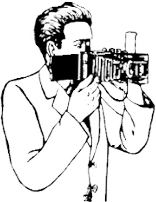
\includegraphics[width=0.4\textwidth]{7-pav}
						\caption{Fotografavimas sulankstomu fotoaparatu}
						\label{fig:7}
					\end{figure}
					\begin{figure}[h]
						\centering
						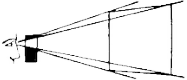
\includegraphics[width=0.4\textwidth]{8-pav}
						\caption{Rėminio vaizdo ieškiklio veikimo principas}
						\label{fig:8}
					\end{figure}

					Rėminis vaizdo ieškiklis (ikonometras) sudarytas iš dviejų rėmelių: mažo ir didelio (negatyvo dydžio); rėmeliai yra nutolę vienas nuo kito atstumu, lygiu objektyvo židinio nuotoliui. Primerkęs vieną akį, antrąja fotografas žiūri pro abu rėmelius. Artindamas akį prie mažojo rėmelio, fotografas randa tokią padėtį, kai visos keturios mažojo rėmelio kraštinės sutampa su visomis keturiomis didžiojo rėmelio kraštinėmis, ir paskui nutaiko aparatą į fotografuojamąjį daiktą. Tuomet visa, kas matyti pro abu rėmelius, išeis ir negatyve (8 pieš.). Rėminis vaizdo ieškiklis rodo vaizdą natūralaus didumo ir yra labai patogus vizuoti. Toks vaizdo ieškiklis yra aparate ``Fotokor'' ir (kaip antrasis vaizdo ieškiklis) aparate ``Liubitel'' (viršutinėje sulankstomojoje šachtoje).

					Atlenkiamas tiesioginis optinis vaizdo ieškiklis sudarytas iš dviejų stačiakampių lęšių: sklaidomojo ir renkamojo (okuliaro), įdėtų į atlenkiamus įtvarus-rėmelius; toks ieškiklis yra fotoaparatuose ``Moskva''.

					Toks pat vaizdo ieškiklis, bet standžios konstrukcijos, su lęšiais, įdėtais į bendrą įtvarą (okuliaras apskritas), montuojamas mažojo formato aparatuose. Laikant fotoaparatą akių lygyje (9 pieš.), pro vaizdo ieškiklio okuliarą matomas labai sumažintas, bet aiškus ir šviesus fotografuojamojo daikto vaizdas.

					Mažojo formato fotoaparatams gaminamas pridedamas universalusis optinis vaizdo ieškiklis (10 pieš.), kurio detalė yra pasukamas skridinys su penkiais įvairiais okuliariniais lęšiais.
					\begin{figure}[h]
						\centering
						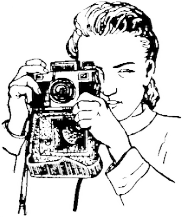
\includegraphics[width=0.4\textwidth]{9-pav}
						\caption{Fotografavimas mažojo formato fotoaparatu}
						\label{fig:9}
					\end{figure}
					\begin{figure}[h]
						\centering
						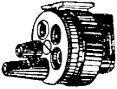
\includegraphics[width=0.4\textwidth]{10-pav}
						\caption{Universalus optinis vaizdo ieškiklis mažojo formato aparatams}
						\label{fig:10}
					\end{figure}
					Pasukus skridinį, vienas iš lęšių įsijungia į optinę vaizdo ieškiklio sistemą, ir ieškiklis rodo tikslų kadrą atitinkamam vienam iš penkių keičiamųjų objektyvų (kurių židinio nuotolis 2,8; 3,5; 5; 8,5 arba 13,5 \textit{cm}).

					Veidrodinis optinis vaizdo ieškiklis (11 pieš.) sudarytas iš dviejų renkamųjų lęšių, iš kurių vienas, mažesnis, įstatytas vertikaliai, o kitas, didesnis, --- horizontaliai viršutinėje vaizdo ieškiklio dalyje; tarp jų 45\degree kampu į abu lęšius įtvirtintas veidrodis, nuo kurio atšoka į viršų spinduliai, praėję pro mažąjį lęšį.
					\begin{figure}[h]
						\centering
						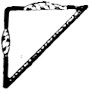
\includegraphics[width=0.4\textwidth]{11-pav}
						\caption{Veidrodinio vaizdo ieškiklio pjūvis}
						\label{fig:11}
					\end{figure}
					Dėl to didysis lęšis sudaro veidrodiškai apverstą fotografuojamojo daikto atvaizdą. Veidrodinis vaizdo ieškiklis blogas tuo, kad į jį žiūrėti reikia iš viršaus, dėl to, naudojant veidrodinį ieškiklį, fotoaparatą tenka laikyti fotgrafo juosmens lygyje (12 pieš.), ir nuotrauka atvaizduoja perspektyvą kiek kitaip, negu paprastai mato mūsų akis. Didelis veidrodinis vaizdo ieškiklis įtaisytas fotoaparato ``Liubitel'' korpuso viršutinėje dalyje.
					\begin{figure}[h]
						\centering
						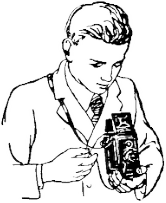
\includegraphics[width=0.4\textwidth]{12-pav}
						\caption{Vizavimas pro dviejų objektyvų fotoaparato veidrodinį vaizdo ieškiklį}
						\label{fig:12}
					\end{figure}
					\begin{figure}[h]
						\centering
						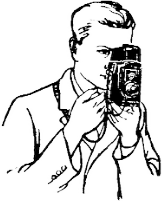
\includegraphics[width=0.4\textwidth]{13-pav}
						\caption{Vizavimas pro dviejų objektyvų fotoaparato rėminį vaizdo ieškiklį}
						\label{fig:13}
					\end{figure}
				\subsubsection*{Kasetės}
					Kasetė yra šviesos nepraleidžiąs metalinis dėklas, į kurį įdėta negatyvinė medžiaga įstatoma į fotoapartą, o po fotografavimo išimama iš jo.

					Plokštelės kasetė --- plokščia, sudaryta iš korpuso ir ištraukiamo dangtelio, į ją telpa viena fotografinė plokštelė. Fotografuojant ji įstatoma į fotoaparatą vietoj matinio stiklo. Aparato ``Fotokor'' kasetės įstumiamos į kameros užpakalinės sienelės išėmas. Aparato ``Moskva 3'' kasetės priglaudžiamos prie kameros užpakalinės sienelės ir pritvirtinamos skląsteliu. Didelių štatyvinių fotokamerų kasetės --- medinės, dvigubos (po vieną plokštelę iš abiejų pusių).

					Mažojo formato fotoaparato filminės juostelės kasetė yra cilindrinės formos, sudaryta iš ritės, korpuso ir dangtelio (FED, ``Zorkij'', ``Zenit'', ``Smena'') arba iš ritės ir dviejų cilindrinių korpuso dalių (``Kijev'', ``Zorkij 3''). Į kasetę telpa 165 \textit{cm} ilgio filminė juostelė --- joje galima padaryti 36 nuotraukas.

					Nuo atsarginių kasečių skaičiaus priklauso, kiek nuotraukų fotografas gali padaryti, negrįždamas į tamsią patalpą.

					Fotoaparatai, skirti plačiam ritiniam filmui, kasečių neturi, filmo juostelė į juos įdedama tiesiog, suvyniota į ritę kartu su šviesos nepraleidžiančiu apsauginiu popieriumi.
			\subsection*{Medžiagos fotografijai}
				\textbf{ŠVIESAI JAUTRIOS MEDŽIAGOS}
				Yra medžiagų, kurios nesikeičia patamsyje, bet tuojau pat pasikeičia, kai jas pasiekia šviesa. Šią savybę (jautrumą šviesai), ir labai ryškią, turi sidabro halogenidai, metalinio sidabro junginiai su vienu iš halogenų --- bromu, chloru ar jodu. Sidabro bromidas, chloridas ir jodidas yra fotografinių sluoksnių jautrusis pagrindas.

				Fotografijai naudojami šviesai jautrūs sluoksniai (arba fotografiniai sluoksniai) --- tai plona želatininė plėvelė, kurioje yra labai daug smulkučių šviesai jautraus sidabro halogenido dalelių (mikrokristalų). Kadangi šis sluoksnis pats yra labai plonas ir nestiprus, jis užliejamas ant stipraus pagrindo: ant siklo (fotografinės plokštelės), ant celiulioido (fotofilmas ir kinofilmas), ant popieriaus (fotografinis popierius).

				Pagal paskirtį šviesai jautrios medžiagos (arba fotografinės medžiagos) skirstomos į negatyvines, naudojamas fotografavimui, ir pozityvines --- atspaudams gaminti.
\end{document}